\documentclass[tikz,border=8pt]{standalone}
\usepackage{tikz}
\usetikzlibrary{arrows.meta,positioning}

\begin{document}
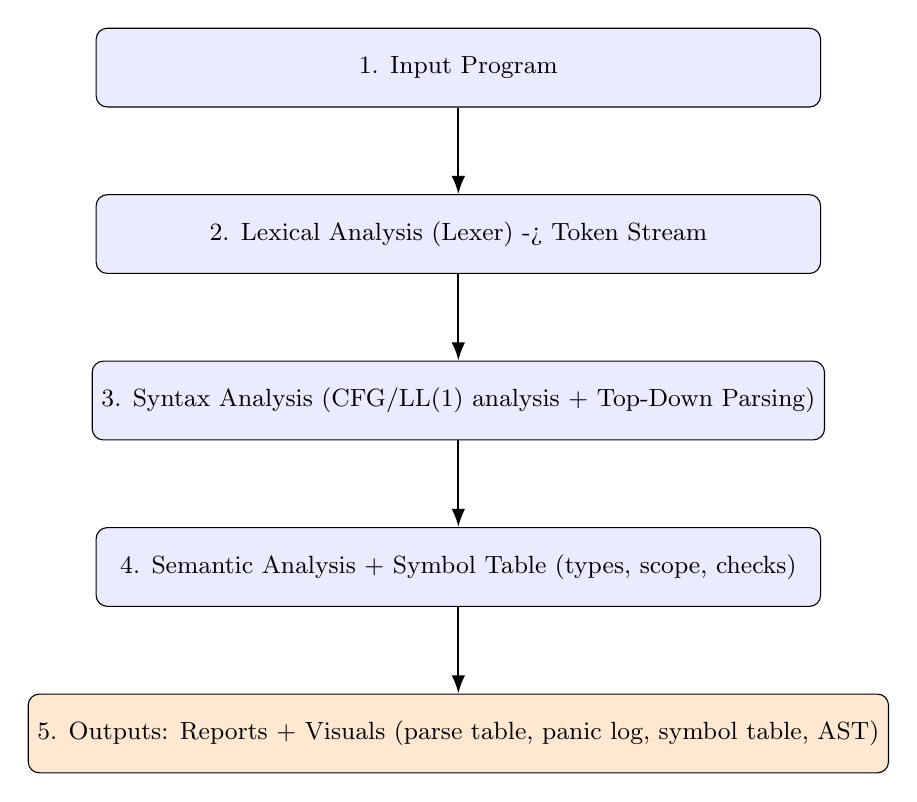
\begin{tikzpicture}[
  font=\small,
  >=Latex,
  node distance=11mm,
  stage/.style={draw, rounded corners, align=center, minimum width=9.2cm, minimum height=10mm, fill=blue!8},
  line/.style={->, thick}
]

% Broad sequential pipeline (5 stages)
\node[stage] (s1) {1. Input Program};
\node[stage, below=of s1] (s2) {2. Lexical Analysis (Lexer) -> Token Stream};
\node[stage, below=of s2] (s3) {3. Syntax Analysis (CFG/LL(1) analysis + Top-Down Parsing)};
\node[stage, below=of s3] (s4) {4. Semantic Analysis + Symbol Table (types, scope, checks)};
\node[stage, below=of s4, fill=orange!18] (s5) {5. Outputs: Reports + Visuals (parse table, panic log, symbol table, AST)};

\draw[line] (s1) -- (s2);
\draw[line] (s2) -- (s3);
\draw[line] (s3) -- (s4);
\draw[line] (s4) -- (s5);

\end{tikzpicture}
\end{document}
